% Section and Frames
\section*{Appendix}
\label{appendix_section}

% Section title frame
\sectiontitleframe{Appendix}

\begin{frame}[fragile]{Preprocessing Step Sequence Randomization I}
    \frametitle{Preprocessing Step Sequence Randomization I}
    \textbf{key points of the Sequence Randomization Feature:}
    \vspace{0.5em}
    \begin{itemize}
        \item A dynamic method to vary the order of preprocessing steps in image preprocessing pipelines.
        \item Preprocessing steps are probabilistically determined, allowing for varied combinations in the pipeline.
        \item Increases flexibility and efficiency in hyperparameter tuning.
    \end{itemize}
\end{frame}

\begin{frame}[fragile]{Preprocessing Step Sequence Randomization II}
    \frametitle{Preprocessing Step Sequence Randomization II}
    \begin{figure}
        \centering
        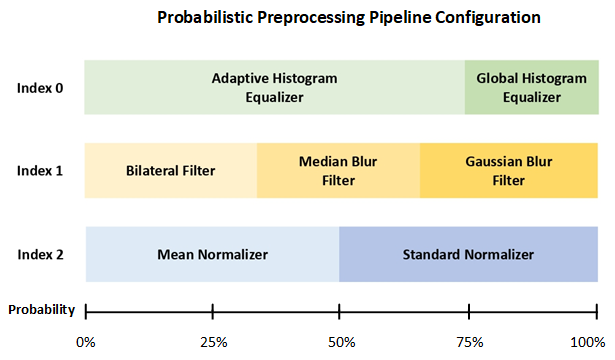
\includegraphics[width=0.8\textwidth]{figures/pipeline_sequence_randomisation_image.png}
        \caption{Illustration of the preprocessing step sequence randomization.}
    \end{figure}
\end{frame}

\begin{frame}[fragile]{Preprocessing Step Sequence Randomization III}
    \frametitle{Preprocessing Step Sequence Randomization III}
    \begin{lstlisting}[label=lst:probabilistic_pipeline_in_json, caption={Probabilistic Pipeline Sequence Definition in JSON Format.}, basicstyle=\scriptsize\ttfamily, stringstyle=\color{black}]
{
    "Adaptive Histogram Equalizer__I0F75": {...Parameters},
    
    "Global Histogram Equalizer__I0F25": {},

    "Bilateral Filter__I1F34": {...Parameters},

    "Median Blur Filter__I1F33": {...Parameters},

    "Gaussian Blur Filter__I1F33": {...Parameters},

    "Standard Normalizer__I2F50": {},

    "Mean Normalizer__I2F50": {},
}
    \end{lstlisting}
\end{frame}

